\section{Columnar database}

A column-oriented database, or columnar database, stores data in columns rather than rows. 
This approach is optimized for Online Analytical Processing (OLAP) and data mining tasks, where efficient read operations over large datasets are essential.

In row-oriented databases, modifying a record is straightforward, but querying might involve reading unnecessary data. 
Columnar databases, however, allow for reading only the relevant columns, making them highly efficient for read-heavy workloads. 
However, writing entire tuples requires multiple column accesses, making columnar databases more suitable for scenarios with high read and lower write demands.
\begin{table}[H]
    \centering
    \begin{tabular}{|l|l|}
    \hline
    \textbf{Advantages}                 & \textbf{Disadvantages}                   \\ \hline
    Data compression                    & Increased disk seek time                 \\ \hline
    Improved bandwidth utilization      & Increased cost of inserts                \\ \hline
    Improved code pipelining            & Increased tuple reconstruction costs     \\ \hline
    Improved cache locality             &                                          \\ \hline
    \end{tabular}
\end{table}
When tuples need to be analyzed, they are often reconstructed using a large prefetch, which helps minimize the effect of disk seeks across columns.

\paragraph*{Compression}
Columnar databases often trade I/O for CPU by leveraging compression techniques more effectively than row-based databases. 
These databases take advantage of higher data value locality in columns, enabling advanced techniques like run-length encoding.
Additional space can be used to store multiple copies of data in different sort orders, further optimizing query performance.

\subsection{Cassandra}
Originally developed by Facebook and now maintained by the Apache Foundation, Cassandra is a popular column-oriented, NoSQL database widely used for high-throughput applications. 

\subsubsection{Architecture}
Cassandra's architecture and its column-oriented approach make it particularly suited for high-availability, large-scale, write-intensive workloads, where distributed, flexible data storage is essential.

Cassandra is masterless since it has no single point of failure. 
Since we have column families based on groups of columns, we have no joins and the data are duplicated. 
The consistency of Cassandra is tunable based on the needs.

\paragraph*{Server mapping}
How do you decide which server(s) a key-value resides on with a masterless approach. 
We design a dependency in a ring form, with the servers connected only with the ring. 

Always a constant amount of network traffic (except for gossip storms)
Simple Strategy
• Single datacenter
• Clockwise placement to the next node(s)
• Network Topology
Strategy
• Multiple datacenters (don't lose all the copies if a datacenter fails)
• Supporting local queries

If a server fails we need to inform the others. 
To avoid using too much bandwith we use gossip protocol: Each node picks its discussants (up to 3)
• Having three messages for each round of gossip adds a degree of anti-entropy.
• This process allows obtaining "convergence" of data shared between
the two interacting nodes much faster
Protocol:
•Nodes periodically gossip
their membership list
•On receipt, the local
membership list is updated






\subsubsection{Data model}
In Cassandra, data is organized into column families, which are analogous to tables in SQL but are more flexible and can have unstructured, client-specified schemas. 
Column Families allow the storage of sparse data, where some columns may be missing in specific rows, fitting Cassandra's NoSQL model.

Each Cassandra keyspace functions similarly to a database, typically used per application with certain configurations set per keyspace. 
The primary elements in Cassandra's data model include:
\begin{enumerate}
    \item \textit{Keyspace}: equivalent to a database, typically unique per application.
    \item \textit{Column family}: groups records of similar types, stored as sparse tables.
    \item \textit{Columns}: each column has three parts:
        \begin{itemize}
            \item \textit{Name}: a byte array used for sorting, querying, and indexing.
            \item \textit{Value}: a byte array; typically not queried directly.
            \item \textit{Timestamp}: used for conflict resolution, with the most recent write winning.
        \end{itemize}
\end{enumerate}
Additionally, Cassandra supports super columns, which group columns under a common name but lack indexing for sub-columns. These are often used to denormalize data from standard column families.
\begin{figure}[H]
    \centering
    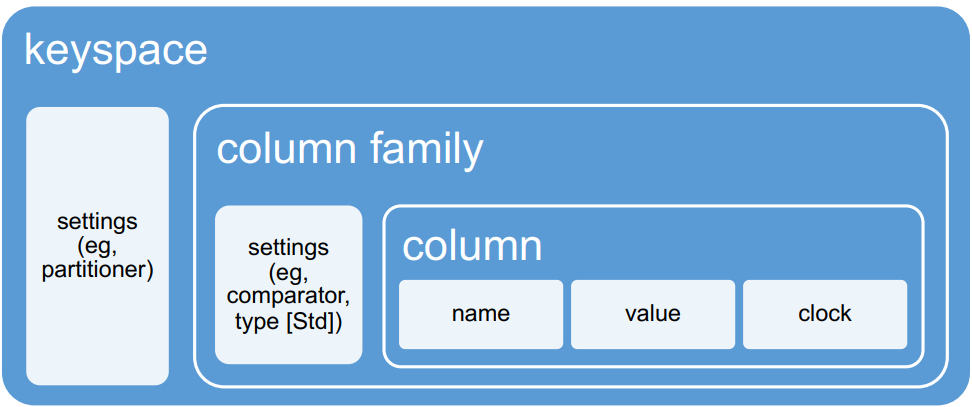
\includegraphics[width=0.75\linewidth]{images/cas.png}
    \caption{Cassandra data model}
\end{figure}

\subsubsection{Query language}
Cassandra supports a unique query mechanism based on a slice predicate, allowing precise control over returned columns:
SliceRange specifies start and end column names, direction (reverse), and count (similar to SQL LIMIT).

To interact with Cassandra, developers can use the API for various read and write operations:
\begin{lstlisting}[style=Java]
// retrieve a specific column at the given path
get() : Column
// retrieve a set of columns in one row specified by the slice predicate
get_slice() : List<ColumnOrSuperColumn>
// retrieve slices for multiple keys based on a SlicePredicate
multiget_slice() : Map<key, List<ColumnOrSuperColumn>>
// retrieve multiple columns according to a specified range
get_range_slices() : List<KeySlice>
\end{lstlisting}
For writing operations, Cassandra provides commands such as:
\begin{lstlisting}[style=Java]
// insert a new element in a column
client.insert()
// update an existing element in a column
batch_mutate()
// remove an existing element from a column
remove()
\end{lstlisting}

\paragraph*{SQL}
Cassandra also supports SQL since it is based in tables with a single column.
The main difference is that in relational databases we have a domain-based model, while in columnar databases we have a query-based model. 
Thus, in this case we start from the queries, and then we design the data model based on that since each column has a key that is used to filter all the elements in the column. 

In case we need to use multiple keys for a family of column we may use an aggregate key, that comprises all the key that may be used in the queries: 
\begin{lstlisting}[style=C]
attribute1:attribute2: { user1, user2}
\end{lstlisting}
We can query based on the first attribute, or both. 

Columns
are sorted according to
\texttt{CompareWith} or \texttt{CompareSubcolumnsWith}

Rows
are placed according to their Partitioner:
•Random: MD5 of key
•Order-Preserving: actual key
are sorted by key, regardless of partitioner